\documentclass{article}

\usepackage{amsmath}
\usepackage{mhchem}
\usepackage{chemfig}
\usepackage{xcolor}
\usepackage{graphicx}
\usepackage[
  left=1cm,
  right=1cm,
  top=2cm,
  bottom=2cm,
]{geometry}

\begin{document}
\section*{Aufgaben - Woche 1}
\subsection*{Aufgabe 1.1}
\begin{equation*}
    p = \frac{nRT}{V}; n=\frac{m}{M}
\end{equation*}
\begin{equation*}
    p = \frac{mRT}{MV}
\end{equation*}
\begin{equation*}
    M = \frac{mRT}{pV} = \frac{2.55 \mathrm{g}\cdot 373.15 \mathrm{K}\cdot\ 8.314 \mathrm{\frac{J}{mol\cdot K}}}{101325 \mathrm{kPa} }= 78.08 \mathrm{\frac{g}{mol}}
\end{equation*}
Für den Stoff mit der Formel \ce{C6H6} ergibt die Molmasse\\$M=6\cdot M(\ce{C})+ 6\cdot M(\ce{H}) = 78.08 \mathrm{\frac{g}{mol}}$ 

\subsection*{Aufgabe 1.2}
Für den Druck gilt:
\begin{equation*}
    p_H=\frac{nRT}{V}=\frac{ 2 \mathrm{mol}\cdot 273.1 \mathrm{K} \cdot 8.135 \mathrm{\frac{J}{mol\cdot K}}}{ 0.0224 \mathrm{m^3}} = 99187 \mathrm{\frac{N}{m}}
\end{equation*}
\begin{equation*}
    p_N= 198375,2 \mathrm{\frac{N}{m}}
\end{equation*}
Die Reaktion läuft nach folgender Gleichung ab:\\
\ce{3H2 + N2 -> NH3}\\
Somit ergibt der Druck nach der vollständigen Umsetzung:
\begin{equation*}
    p_{Ges}=\frac{3}{4}p_H + \frac{1}{4}p_N = 198375,2 \frac{\mathrm{N}}{\mathrm{m}}
\end{equation*}
\\
Korrekte Lösung:
\begin{center}
    \begin{tabular}{c c c c}
        \hline
        - & $n_H$ & $n_N$ $n_{NH3}$\\
        \hline
        vor: & 2 mol & 1 mol & -\\
        Reakt: & 2 mol & $\frac{2}{3}$ mol & $\frac{4}{3}$ mol\\
        nach: & - & $\frac{1}{3}$ mol & $\frac{4}{3}$ mol\\ 
        \hline
    \end{tabular}
\end{center}
\begin{equation*}
    n_{ges}=\frac{1}{3} + \frac{4}{3} = \frac{5}{3} ( \mathrm{mol})
\end{equation*}
\begin{equation*}
    p_{ges} = 1,69 \cdot 10^5 Pa
\end{equation*}
\begin{equation*}
    x_i = \frac{n_i}{n_{ges}}
\end{equation*}
\begin{equation*}
    x_H = 0; x_N = \frac{\frac{1}{3}}{\frac{5}{3}}; x_{NH3}=0,8
\end{equation*}
\begin{equation*}
    p_i = x_i \cdot p_{ges}
\end{equation*}
Damit berechnen.

\subsection*{Aufgabe 1.3}
a)
\begin{equation*}
    dp = \left(\frac{\partial p}{\partial V}\right)_T dV + \left(\frac{\partial p}{\partial T}\right)_V dT
\end{equation*}
b)
\begin{equation*}
    d^2p=\frac{2nR}{V^3}d^2V-2\frac{nR}{V^2}dTdV
\end{equation*}
Schwartzschen Satz beweisen:
\begin{equation*}
    \frac{\partial^2 p}{\partial V \partial T} = \frac{\partial^2 p}{\partial T \partial V}
\end{equation*}
\begin{equation*}
    -\frac{nr}{V^2} = -\frac{nr}{V^2} 
\end{equation*}

\subsection*{Aufgabe 1.4}
a)
\begin{equation*}
    \alpha = \frac{1}{V}\left(\frac{\partial V}{\partial T}\right)_p = \frac{1}{\frac{nRT}{p}} \cdot \frac{nR}{p} = \frac{1}{T}
\end{equation*}
\begin{equation*}
    \beta = \frac{1}{p}\left(\frac{\partial p}{\partial T}\right)_V = \frac{1}{\frac{nRT}{V}} \cdot \frac{nR}{V} = \frac{1}{T}
\end{equation*}
\begin{equation*}
    K = -\frac{1}{V}\left(\frac{\partial V}{\partial p}\right)_V = -\frac{1}{\frac{nRT}{V}} \cdot -\left(\frac{nRT}{p^2}\right) = \frac{1}{p}
\end{equation*}
b)
\begin{equation*}
    \alpha = \beta K p
\end{equation*}
\begin{equation*}
    \frac{1}{V}\left(\frac{\partial V}{\partial T}\right)_p = \left(\frac{\partial p}{\partial T}\right)_V\cdot \left(-\frac{1}{V}\right)\left(\frac{\partial V}{\partial p}\right)_T
\end{equation*}
\begin{equation*}
    \left(\frac{\partial V}{\partial T}\right)_p = -\left(\frac{\partial p}{\partial T}\right)_V \left(\frac{\partial V}{\partial P}\right)_T   |\cdot \left(\frac{\partial T}{\partial V}\right)_P
\end{equation*}
\begin{equation*}
    \left(\frac{\partial V}{\partial T}\right)_p \left(\frac{\partial T}{\partial V}\right)_p = -\left(\frac{\partial p}{\partial T}\right)_V \left(\frac{\partial V}{\partial P}\right)_T \left(\frac{\partial T}{\partial V}\right)_P
\end{equation*}
Da gilt:
\begin{equation*}
    \left(\frac{\partial V}{\partial T}\right)_p\left(\frac{\partial p}{\partial T}\right)_V\left(\frac{\partial V}{\partial p}\right)_T = -1 ; \left(\frac{\partial V}{\partial T}\right)_p \left(\frac{\partial T}{\partial V}\right)_p = 1
\end{equation*}
Ergibt dies:
\begin{equation*}
    1 = 1
\end{equation*}

\subsection*{Aufgabe 1.5}
\begin{equation*}
    \lambda = \frac{\langle v \rangle}{z_1}=\frac{1}{\sqrt{2}\sigma \frac{N}{V}}=\frac{1}{\sqrt{2}\sigma \frac{p}{K_BT}}
\end{equation*}
Auf diese GLeichung kommt man mit folgenden Umformungen:
\begin{equation*}
     z_1 = \sqrt{2} \langle v \rangle \sigma \frac{N}{V}
\end{equation*}
\begin{equation*}
    pV = nRT | n = \frac{N}{N_A}
\end{equation*}
\begin{equation*}
    pV = \frac{N}{N_A} RT = NK_BT
\end{equation*}
\begin{equation*}
    p = \frac{N}{V}K_BT
\end{equation*}
\begin{equation*}
    \frac{N}{V} = \frac{p}{K_BT}
\end{equation*}
Somit:
\begin{equation*}
    \lambda_N = 6.76 \cdot 10^{-5} \mathrm{m}
\end{equation*}

\subsection*{Aufgabe 1.6}
\begin{equation*}
    T_1 = 273.15 \, \mathrm{K}, T_2 = 373.15 \, \mathrm{K}
\end{equation*}
\begin{equation*}
    p_1 = p_2
\end{equation*}
\begin{equation*}
    \frac{n_1 R T_1}{V} = \frac{n_2 R T_2}{V}
\end{equation*}
\begin{equation*}
    n_1 T_1 = n_2 T_2
\end{equation*}
\begin{equation*}
    n_1 + n_2 = n = 2 \, \mathrm{mol}
\end{equation*}
\begin{equation*}
    n_1T_1=(2-n_1)T_2
\end{equation*}
\begin{equation*}
    n_1T_1=2T_2-n_1T_2
\end{equation*}
\begin{equation*}
    n_1(T_1+T_2)=2T_2
\end{equation*}
\begin{equation*}
    n_1\frac{2T_2}{T_1 + T_2} = 0.845 \, \mathrm{mol}
\end{equation*}
\begin{equation*}
    n_2 = 2 - n_1 = 1.155 \, \mathrm{mol}
\end{equation*}
\begin{equation*}
    p = \frac{n_1RT_1}{V} = 1.072 \cdot 10^5 \, \mathrm{Pa}
\end{equation*}

\subsection*{Aufgabe 1.7}
\begin{equation*}
    E_{pot} = 4\varepsilon\left(\left(\frac{r_0}{r}\right)^{12} - \left(\frac{r_0}{r}\right)^6\right)
\end{equation*}
\begin{equation*}
    F = \frac{dE_{pot}}{dr}=\left(\left(-12\cdot 4\varepsilon r_0^{12} \cdot r^{-13}\right)-\left(-6\cdot 4\varepsilon r_0^6r^{-7}\right)\right)
\end{equation*}
\begin{equation*}
    \frac{48\varepsilon r_0^{12}}{r^13} - \frac{24\varepsilon r_0^6}{r^7} = 0
\end{equation*}
damit:
\begin{equation*}
    0 = \frac{2 r_0^12}{r^13}-\frac{r_0^6}{r^2}
\end{equation*}
Damit:
\begin{equation*}
    r_0^6r^6 = 2r_0^12
\end{equation*}
\begin{equation*}
    r = \sqrt[6]{2}r_0
\end{equation*}
\begin{equation*}
    r^6=\frac{2r_0^{12}}{r_0^6}=2r_0^6
\end{equation*}
\begin{equation*}
    r=\sqrt[6]{2}r_0
\end{equation*}
\begin{equation*}
    E_{pot}=-\varepsilon
\end{equation*}

\section*{Aufgaben - Woche 2}
\subsection*{Aufgabe 2.1}
Wird die Virialgleichung nach dem zweiten Glied abgebrochen lautet diese:
\begin{equation*}
    \frac{pV_m}{RT} = 1+B_pp
\end{equation*}
Mit den ersten Werten $p = 1.013$ bar und $pV_m = 22.693\,\mathrm{\frac{bar}{mol}}$, ergibt sich:
\begin{equation*}
    \frac{22.693\,\mathrm{\frac{bar}{mol}}}{8.3145\,\mathrm{\frac{J}{molK}}\,\cdot273\,\mathrm{K}} = 1 + B_p \cdot 1.013 \,\mathrm{bar} \rightarrow B_p = -0.977\,\mathrm{J}
\end{equation*}
\begin{center}
    \begin{tabular}{c c c}
        \hline
        $p$ [bar] & $pV_m$ [$\mathrm{\frac{bar}{mol}}$] & $B_p$ [J]\\
        \hline
        1.013&22.693&-0.9772\\
        3.039&22.673&-0.3256\\
        5.065&22.652&-0.1955\\
        \hline
    \end{tabular}
\end{center}
Mit der Gleichung
\begin{equation*}
    T_B \approx \frac{a}{bR}
\end{equation*}
mit den Van-der-Waals-Koeffizienten $a(\ce{N2}) = 140.8\cdot 10^{-3}\,\mathrm{\frac{Jm^3}{mol^2}}$ und $b(\ce{N2})=39.1\cdot 10^{-6}\,\mathrm{\frac{m^3}{mol}}$
\begin{equation*}
    T_B = 433.10\,\mathrm{K} < 273\,\mathrm{K}
\end{equation*}
Somit liegt die Messtemperatur unter der Boyletemperatur $T_B$.

\subsection*{Aufgabe 2.2}
\begin{equation*}
    p = \frac{nRT}{V-nb} - a \left(\frac{n}{V}\right)^2 = \frac{1\cdot 8.3145 \cdot 200}{0.005 - 1 \cdot 39.13 \cdot 10^{-6}}-140,8\cdot 10^{-3}\left(\frac{1}{0.005}\right)^2 \,\mathrm{bar} = 329.5740\,\mathrm{kbar}
\end{equation*}
\begin{equation*}
    p = \frac{nRT}{V} \rightarrow p = \frac{1\cdot 8.3145 \cdot 200}{0.005}\,\mathrm{bar} = 332.5800\,\mathrm{kbar}
\end{equation*}
Da der Druck nach der VdW Gleichung kleiner ist als nach der idealen Gasgleichung ist davon auszugehen, dass die anziehenden Kräfte zwischen den Molekülen überwiegt, dafür spricht auch das typische Verhalten bei kleinem $T$ und $B_p < 0$

\subsection*{Aufgabe 2.3}
a)
\begin{equation*}
    p = \frac{RT}{V_m-b}-\frac{a}{V_m^2}
\end{equation*}
\begin{equation*}
    \frac{\partial p}{\partial V_m} = 0, \, \frac{\partial^2 p}{partial V_m^2}=0
\end{equation*}
\begin{equation*}
    \frac{\partial p}{\partial V_m} = \frac{RT}{(V_m-b)^2}+\frac{2a}{V_m^3}=0 \Rightarrow \frac{2}{(V_m-b)}\frac{2a}{V_m^3} = \frac{6a}{V_m^4}
\end{equation*}
\begin{equation*}
    \frac{\partial^2 p}{\partial V_m^2} = \frac{2RT}{(V_m-b)^3}-\frac{6a}{Vm^4}=0 \Rightarrow \frac{2}{V_m-b}=\frac{3}{V_m}
\end{equation*}
\begin{equation*}
    V_{m,krit} = 3b
\end{equation*}
Daraus folgt:
\begin{equation*}
    T_{krit} = \frac{2a(V_m-b)^2}{V_m^3\cdot R}=\frac{8a}{27Rb}
\end{equation*}
\begin{equation*}
    p_{krit} = \frac{\frac{8a}{b}}{3b-b}-\frac{a}{9b^2} = \frac{a}{27b^2}
\end{equation*}
b)
\begin{equation*}
    T_{krit} = 304,01 \,\mathrm{K}
\end{equation*}
c)
\begin{equation*}
    \left(p_r\frac{3}{V_r^2}\right) = \frac{\frac{8T_r}{3}}{\left(V_r-\frac{1}{3}\right)}
\end{equation*}
\begin{equation*}
    \left(p_r\frac{3}{V_r^2}\right)\left(V_r-\frac{1}{3}\right) = \frac{8}{3}T_r
\end{equation*}

\subsection*{Aufgabe 2.4}
\begin{equation*}
    p = \frac{RT}{Vm}-\frac{B}{V_m^2}+\frac{C}{V_m^3}
\end{equation*}
\begin{eqnarray*}
    p' = -RTV_m^{-2}+2BV_m^{-3}-3CV_m^{-4} = 0\\
    p'' = 2RTV_m^{-3}-6BV_m^{-4}+12CV_m^{-5} = 0
\end{eqnarray*}
Die beiden miteinander verrechnet ergibt:
\begin{eqnarray*}
    (4B-6B)V_m+12C-6C = 0\\
    -2BV_m+6C=0\\
    V_{m,krit} = \frac{3C}{B}
\end{eqnarray*}

\subsection*{Aufgabe 2.5}
\begin{eqnarray*}
    \frac{pV_m}{RT}=1+B_pp+C_pp^2\\
    \frac{pV_m}{RT}=1+\frac{B_V}{V_m}+\frac{C_V}{V_m^2}
\end{eqnarray*}
Die zweite Gleichung nach p umgestellt ergibt:
\begin{equation*}
    p = \frac{RT}{V_m}+\frac{B_VRT}{V_m}+\frac{C_VRT}{V_m^3}
\end{equation*}
\begin{equation*}
    \frac{pV_m}{RT}=1+\frac{B_pRT}{V_m}+\frac{B_pB_VRT}{V_m^2}+\frac{B_pC_VRT}{V_m^3}+C_p\left(\frac{RT}{V_m}+\frac{B_VRT}{V_m^2}+\frac{C_VRT}{V_m^3}\right)\cdot\left(\frac{RT}{V_m}+\frac{B_VRT}{V_m^2}+\frac{C_VRT}{V_m^3}\right)
\end{equation*}
\begin{eqnarray*}
    \frac{pV_m}{RT}\approx 1 + \frac{B_pRT}{V_m}+\frac{B_pB_vRT}{V_m^2}+\frac{C_p(RT)^2}{V_m^2}\\
    =1+\frac{B_pRT}{V_m}+\frac{RTB_pB_V+C_p(RT)^2}{V_m^2}
\end{eqnarray*}
Somit ist $\frac{B_pRT}{V_m} = B_V$ und $\frac{RTB_pB_V+C_p(RT)^2}{V_m^2} = C_V$
\begin{eqnarray*}
    = B_V^2+C_p(RT)^2\\
    C_V - B_V^2 = C_p(RT)^2\\
    C_p = \frac{C_V-B_V^2}{(RT)^2}
\end{eqnarray*}

\subsection*{Aufgabe 2.6}
a)
\begin{equation*}
    w = -\int_{V_A}^{V_E} p\,dV = -nRT\ln\left(\frac{V_E}{V_A}\right) = -1\cdot 8.3145 \cdot 273 \cdot \ln\left(\frac{0.0448}{0.0224}\right) \,\mathrm{J}= -1573,3460 \,\mathrm{J}
\end{equation*}
\\b)
\begin{equation*}
    -p_{ex}\Delta V = -\frac{RT}{V} \cdot 0.0224\,\mathrm{m^3}=-1135.5528\,\mathrm{J}
\end{equation*}
\\c)
\begin{equation*}
    w = 0
\end{equation*}

\subsection*{Aufgabe 2.7}
\begin{eqnarray*}
    \partial w = -p\,dV\\
    dV = \left(\frac{\partial V}{\partial T}\right)_p\,dT + \left(\frac{\partial V}{\partial p}\right)_T\,dp,\,V=\frac{nRT}{p}\\
    \left(\frac{\partial V}{\partial T}\right)_p = \frac{nR}{p}\\
    \left(\frac{\partial V}{\partial p}\right)_T = \frac{-nRT}{p^2}\\
    \partial w = -p\frac{nR}{p}\,dT + p \frac{nRT}{p^2}dp = -nR\,dT + \frac{nRT}{p}\,dp\\
    \left(\frac{\partial w}{\partial T}\right)_p = -nR,\, \left(\frac{\partial w}{\partial p}\right)_T = \frac{nRT}{p}\\
    \left(\frac{\partial^2 w}{\partial T \partial p}\right) = \frac{\partial}{\partial p}\left(\frac{nRT}{p}\right)=\frac{nR}{p}\\
    \frac{\partial^2 w}{\partial p \partial T} = \frac{\partial}{\partial p}(-nR) = 0\\
    \frac{\partial^2 w}{\partial T \partial p} = \frac{\partial^2 w}{\partial p \partial T} \Rightarrow \partial w
\end{eqnarray*}
$w$ ist keine Zustandsgröße

\section*{Woche 3}
\subsection*{Augabe 3.1}
a)\begin{eqnarray*}
    V=\mathrm{const.},\,w=0\\
    q_v=nc_{m,V}\Delta T\\
    c_p=c_V+nR \rightarrow c_{v,m} = c_{p,m} - R\\
    q_V=(c_{p,m}-R)n\Delta T = 124.76\,\mathrm{J}
\end{eqnarray*}
Es wird keine Arbeit verrichtet\\
b)\begin{eqnarray*}
    p = \mathrm{const.}\\
    q_p=nc_{p,m}\Delta T = 207.9\,\mathrm{J}\\
\end{eqnarray*}
\begin{equation*}
    w=-p\Delta V \ce{->[{pV=nRT}]} -p(\frac{nRT_E}{p}-\frac{nRT_A}{p})=-nr\Delta T = -83.14\,\mathrm{J}
\end{equation*}

\subsection*{Aufgabe 3.2}
\begin{eqnarray*}
    q_K=C\Delta T,\,V=\mathrm{const.}\\
    q_V=\Delta U=-C\Delta T = n \Delta U_m = \frac{m}{M} \Delta U_m\\
    \Delta U_m = -\frac{C\Delta TM}{m}=-3261.96\,\mathrm{J}
\end{eqnarray*}
\begin{eqnarray*}
    H=U+pV\\
    \Delta H=\Delta U + \Delta (pV) = \Delta U + p \Delta V \rightarrow[{p\Delta V = \Delta n_gRT}]\rightarrow \Delta U + \Delta n_g RT\\
    \Delta n_g = (6-7.5)\,\mathrm{mol} = -1.5\,\mathrm{mol}\\
    \Delta H_m = -3265.7\cdot 10^3 \,\mathrm{\frac{J}{mol}}
\end{eqnarray*}

\subsection*{Aufgabe 3.3}
\begin{eqnarray*}
    \mu = \left(\frac{\partial T}{\partial p}\right)_H
    d H_m = \left(\frac{\partial H_m}{\partial T}\right)_p\,dT+\left(\frac{\partial H_m}{\partial p}\right)_T\,dp=C_{p,m}\,dT+\left(\frac{\partial H_m}{\partial p}\right)_T\,dp\\
    \text{mit: } \left(\frac{\partial H_m}{\partial p}\right)_T = -T\left(\frac{\partial V_m}{\partial T}\right)_p + V_m\\
    c_{p,m}\,dT+\left[-T\left(\frac{\partial V_m}{\partial T}\right)_p+V_m\right]\,dp=0\\
    \mu = \left(\frac{\partial T}{\partial p}\right)_H = \frac{1}{C_{p,m}}\left[T\left(\frac{\partial V_m}{\partial T}\right)_p - V_m\right]
\end{eqnarray*}
a)\begin{eqnarray*}
    pV_m-pb=RT\\
    V_m = \frac{RT}{p}+b\\
    \left(\frac{\partial V_m}{\partial T}\right)_p = \frac{R}{p}\\
    \mu = \frac{1}{c_{p,m}}\left[T\frac{R}{p}-\left(\frac{RT}{p}+b\right)\right]=-\frac{b}{c_{p,m}}<0\\
\end{eqnarray*}
b)\begin{eqnarray*}
    pV_m=RT+(b-\frac{a}{RT})_p\\
    V_m = \frac{RT}{p}+b-\frac{a}{RT}\\
    \left(\frac{\partial V_m}{\partial T}\right)_p = \frac{R}{p}+\frac{a}{RT^2}\\
    \mu = \frac{1}{c_{p,m}}\left[-\left(\frac{R}{p}+\frac{a}{RT^2}\right)-\left(\frac{RT}{p}+b-\frac{a}{RT}\right)\right]\\
    = \frac{1}{c_{p,m}}\left(\frac{2a}{RT}-b\right)
\end{eqnarray*}
\subsection*{Aufgabe 3.4}
\begin{center}
    I. \ce{(Cyclohexan) + 18 O2 -> 6CO2 + 6H2O}\\
    II. \ce{(Cyclohexen) + 16 O2 -> 6CO2 + 5H2O}\\
    III. \ce{(Cyclohexa-1,3-dien) + 14 O2 -> 6CO2 + 4H2O}\\
    IV. \ce{(Benzol) + 12 O2 -> 6CO2 + 3H2O}
\end{center}
I.
\begin{eqnarray*}
    6\cdot\Delta_BH^0_m(\ce{CO2})+6\cdot\Delta_BH^0_m(\ce{H2O})-\Delta_BH^0_m(\mathrm{Cyclohexan})\\
    6\cdot -395.5 + 6 \cdot -285.9 + 156.2\,\mathrm{\frac{kJ}{mol}} = -3932.2\,\mathrm{\frac{kJ}{mol}}\\
\end{eqnarray*}
Analog:\\
II. gegeben: $-3739.0\,\mathrm{\frac{kJ}{mol}}$\\\\
III $-3623.6\,\mathrm{\frac{kJ}{mol}}$\\\\
IV $-3279.74\,\mathrm{\frac{kJ}{mol}}$\\\\
Hydrierungsenthalpien:\\
II:
\begin{equation*}
    -3739 + 3932.2 \,\mathrm{\frac{kJ}{mol}}= 193.2\,\mathrm{\frac{kJ}{mol}}
\end{equation*}
III:
\begin{equation*}
    -3623.6 + 3739 \,\mathrm{\frac{kJ}{mol}}= 116\,\mathrm{\frac{kJ}{mol}}
\end{equation*}
IV:
\begin{equation*}
    -3279.74 + 3623.6 \,\mathrm{\frac{kJ}{mol}}= 343.86\,\mathrm{\frac{kJ}{mol}}
\end{equation*}
\subsection*{Aufgabe 3.5}
\begin{eqnarray*}
    \Delta_RH^0(600)=\Delta_RH^0(298.15)+(0.001(6\cdot 36 + 4\cdot 29 - 5 \cdot 29 - 4\cdot 42))\Delta T \,\mathrm{\frac{kJ}{mol}}= -904.6 \cdot 0.019 \cdot 301.85 \,\mathrm{\frac{kJ}{mol}} = -5188.0167\,\mathrm{\frac{kJ}{mol}}
\end{eqnarray*}

\section*{Woche 4}
\subsection*{Aufgabe 4.1}
a)
\begin{center}
    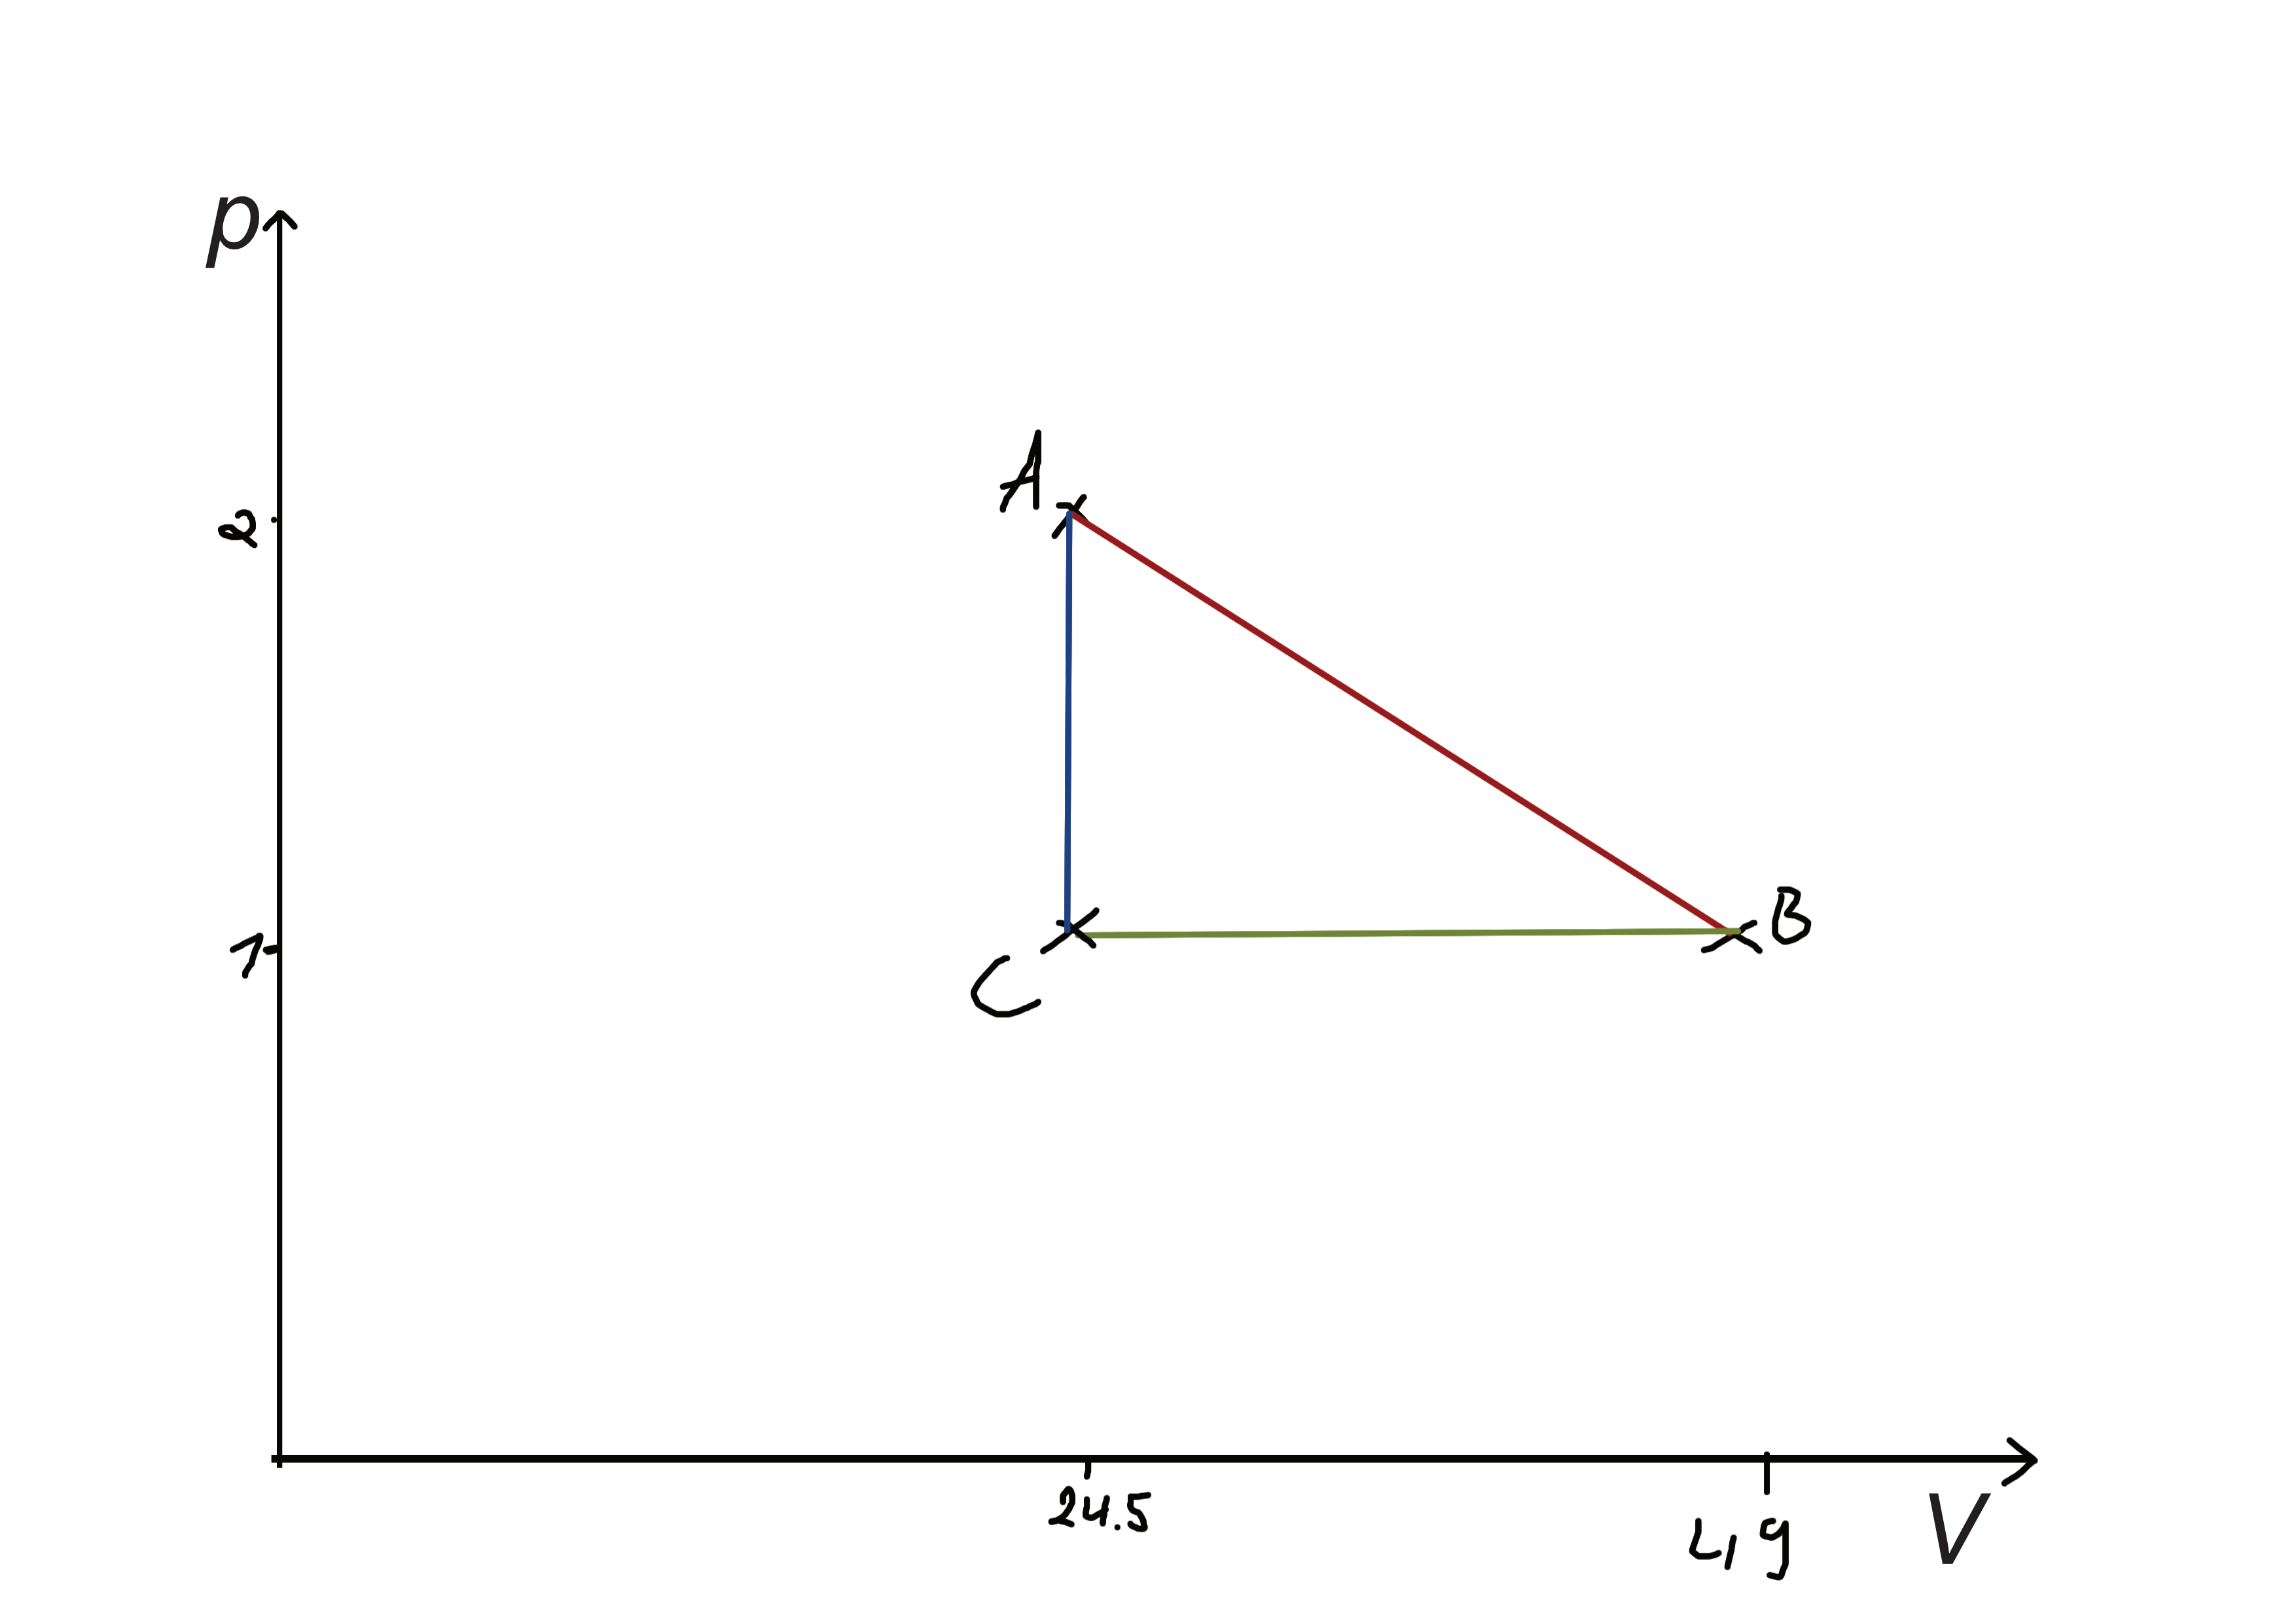
\includegraphics[width=500pt]{img/What.png}
\end{center}
b)\begin{eqnarray*}
    V_A = 24.5\,\mathrm{l}\\
    V_B = 49\,\mathrm{l}\\
    T_A = 298\,\mathrm{K}\\
    T_B = 298\,\mathrm{K}\\
    p_AV_A=p_BV_B (T=\mathrm{const.})\\
    p_B=\frac{p_AV_A}{V_B}=\frac{p_A}{2} = \frac{2\,\mathrm{bar}}{2} = 1\,\mathrm{bar}\\\\
    B\rightarrow C\\
    p = \mathrm{const} p_C = 1\,\mathrm{bar}\\\\
    C\rightarrow A (q = 0)\\
    p_AV_A^\gamma = p_CV_C^\gamma\\
    \gamma = \frac{C_{p,m}}{C_{V,m}} = \frac{C_{V,m}+R}{C_{v,m}} = \frac{\frac{5R}{2}+R}{\frac{5R}{2}} = \frac{7}{5}= 1,4
    V_C = V_A \left(\frac{p_A}{p_C}\right)^\frac{1}{\gamma} = 24.5\,\mathrm{l}\cdot 2^\frac{1}{1.4} = 40.2\,\mathrm{l}\\\\
    B\rightarrow C\\
    \frac{V_C}{V_B} = \frac{T_C}{T_B}\\
    T_C = \frac{T_BV_C}{V_B} = 244.5\,\mathrm{K}\\
    T_V = \frac{p_CV_C}{nR}\\
    n=\frac{p_AV_A}{RT_A} = 1.978\,\mathrm{mol}
\end{eqnarray*}
c)\begin{eqnarray*}
    A\rightarrow B\\
    T =\mathrm{const},\,\Delta U_1 = 0 = q_1+w_1 \Rightarrow w_1 = -q_1\\
    w_1 = -nRT_A\ln\frac{V_B}{V_A} = -p_AV_A\ln 2 = -2\cdot 10^5 \,\mathrm{Pa} \cdot 24.5\,cdot 10^{-3}\,\mathrm{m^3}\ln 2 = -3396,42\,\mathrm{J}\\
    q_1=3396,42\,\mathrm{J}\\\\
    B\rightarrow C\\
    p = \mathrm{const.}\\
    w_2 = -p_B(V_C-V_B)=-10^5\,\mathrm{Pa}(40.2-49)\cdot 10^{-3}\,\mathrm{m^3} = 880.4\,\mathrm{J}\\
    q_2 = nC_{p,m}(T_C-T_B) = \frac{7}{2}\cdot 8.314\,\mathrm{\frac{J}{mol\cdot K}}\cdot 1.978\,\mathrm{mol}(244.5-298)\,\mathrm{K} = -3081.6\,\mathrm{J}\\
    C_{p,m}=C_{V,m}+R = \frac{7R}{2}\\\\
    C\rightarrow A\\
    q_3 = 0,\, \Delta U_3 = w_3 = nC_{V,m}(T_A-T_C)=2201.18\,\mathrm{J}
\end{eqnarray*}
d)\begin{eqnarray*}
    \eta = \frac{|w_{Ges|}}{q_1}\\
    w_{Ges} = 2_1 + w_2 + w_3 = -314.8\,\mathrm{J}\\
    \eta = \frac{314.8\,\mathrm{J}}{3396.42\,\mathrm{J}} = 0.093 = 9.3\,\%
\end{eqnarray*}

\subsubsection*{Aufgabe 4.2}
\begin{eqnarray*}
    dS = \frac{\delta q_{rev}}{T},\, \delta q =\frac{nRT}{V}dV\\
    dS = \frac{1}{T}\left(\frac{nRT}{V}dV\right)\\
    \Delta S = nR \int_{V_A}^{V_E}\frac{1}{V}dV\\
    = nR \ln \frac{V_E}{V_A}\\
    \Delta S = \Delta S_A + \Delta S_B\\
    =n_A R\ln \left(\frac{V_{ges}}{V_A}\right)+n_BR\ln\left(\frac{V_{ges}}{V_B}\right),\, p_V = nRT \Rightarrow V = \frac{nRT}{p}\\
    =n_AR\ln\left(\frac{n_{ges}}{n_A}\right)+n_BR\ln\left(\frac{n_{ges}}{n_A}\right)\\\\
    B:
    \Delta S = 4.16\,\mathrm{\frac{J}{K}}\\
    \text{Wenn nicht gleich 0, irreversibel}\\
\end{eqnarray*}

\subsection*{Aufgabe 4.3}
\begin{eqnarray*}
    T_W =\frac{T_1+T_2}{2}\\
    \Delta S_{Sys} = \Delta S_1 + \Delta S_2\\
    = \int_{T_1}^{T_E}C_p\,dT + \int_{T_1}^{T_E}C_p\,dT\\
    C_P\ln\frac{T_2}{T_1}+C_p\ln\frac{T_E}{T_2} \text{ für} T_E \text{ in vorheriger Gleichung einsetzen}\\
    C_p\ln\frac{T_E^2}{T_1T_2}=C_p\ln\frac{\left(T_1+T_2\right)^2}{4T_1T_2}\\
    \Delta S_{Umg} = 0\\
    \frac{\ln\left(T_1 + T_2\right)^2}{4T_1T_2}\\\text{Der obere Teil im ln muss größer 1 sein, damit der gesamte obere Teil des Bruches größer als 1 wird}\\
    (T_1 + T_2)^2 > 4T_1T_2\\
    T_1^2+2T_1T_2+T_2^2 > 4T_1T_2\\
    (T_1 - T_2)^2 > 0\\
    T_1 \neq T_2
\end{eqnarray*}

\subsubsection*{Aufgabe 4.4}
a)\begin{eqnarray*}
    \Delta S_m = -\Delta_{S,m} H_m^{273}=\frac{-6000\,\mathrm{\frac{J}{mol}}}{273.15\,\mathrm{K}}=-21.97\,\mathrm{\frac{J}{mol\cdot K}}\\
    \Delta_{einfrieren}H = -\Delta_{s,m}H\\
    \Delta S_{Umg} = 21.97\,\mathrm{\frac{J}{mol\cdot K}}\\
    \Delta S_{Ges} = 0
\end{eqnarray*}
b)\begin{align*}
    \Delta S &=C_p\ln\frac{T_E}{T_A}\\
    \Delta S &= \Delta S_{1,m} + \Delta S_{2,m} + \Delta S_{3,m} = C_{p,m}\ln\frac{T_2}{T_1}-\frac{\Delta_{s,m}H^{273}}{T_2}+C_{p,m}\ln\frac{T_1}{T_2}\\
    &=75\,\mathrm{\frac{J}{mol\cdot K}}\ln\frac{273.15}{263.15}-21.97\,\,mathrm{\frac{J}{mol\cdot K}}+38\,\mathrm{\frac{J}{mol\cdot K}}\ln\frac{263.15}{273.15}=-20.59\,\mathrm{\frac{J}{mol\cdot K}}\\
    \mathrm{Umgebung}:\\
    \Delta S_{Umg} &= \frac{\Delta_{s,m} H ^{263}}{T_1} = \frac{5630\,\mathrm{\frac{J}{mol\cdot K}}}{263.15\,\mathrm{K}}=21.395\,\mathrm{\frac{J}{mol\cdot K}}\\
    \Delta S_{Ges} &= 0.8\,\mathrm{\frac{J}{mol\cdot K}}
\end{align*}

\section*{Woche 5}
\subsection*{Aufgabe 5.1}
1) Eis -10 °C auf 0 °C
\begin{eqnarray*}
    q_1 = nC_{p,m}\Delta T\\
    n = \frac{m}{M} = \frac{1000}{18} = 55.556\,\mathrm{mol}\\
    q_1 = 55.556\,\mathrm{mol}\cdot 38\,\mathrm{\frac{J}{mol\cdot K}}\cdot 10\,\mathrm{K}=21.1\,\mathrm{kJ}
\end{eqnarray*}
2)
\begin{eqnarray*}
    q_2 = n\Delta H_{schmelz,s}^{Eis} = 333,3\,\mathrm{kJ}
\end{eqnarray*}
3) Wasser 0 °C auf 100 °C
\begin{eqnarray*}
    q_3 = nC_{p,m}^{Wasser}\Delta T =419.4\,\mathrm{kJ}
\end{eqnarray*}
4) Verdampfen
\begin{eqnarray*}
    q_4 = n \Delta H_{verd,m}1{Wasser} = 2277.8\,\mathrm{kJ}
\end{eqnarray*}
5) Dampf 100 °C auf 150 °C
\begin{eqnarray*}
    q_5 = nC_{p,m}^{Dampf} \Delta T = 
\end{eqnarray*}
\begin{equation*}
    q_{\sum} = q_1 + q_2 + q_3 + q_4 + q_5 = 3146\,\mathrm{kJ}
\end{equation*}
\begin{align*}
    \Delta S &= n C_{p,m} \ln\frac{T_E}{T_A}\text{ Erwärmen}\\
    \Delta S &= \frac{n\Delta H}{T}=\frac{q}{T}\text{ Phasenübergang}\\
    \Delta S_1 &= 78.8\,\mathrm{\frac{J}{K}}\\
    \Delta S_2 &= 1221\,\mathrm{\frac{J}{K}}\\
    \Delta S_3 &= 1309.1\,\mathrm{\frac{J}{K}}\\
    \Delta S_4 &= 6106.6\,\mathrm{\frac{J}{K}}\\
    \Delta S_5 &= 237.6\,\mathrm{\frac{J}{K}}\\
    \Delta S_{\sum} &= 8953.1\,\mathrm{\frac{J}{K}}
\end{align*}
\subsection*{Aufgabe 5.2}
\begin{align*}
    C &= a+bT\\
    T_1 &= 373\,\mathrm{K}\\
    T_2 = 573\,\mathrm{K}\\
\end{align*}
a)
\begin{align*}
    \Delta H &= a(T_2-T_1)+\frac{b}{2}(T_2^2-T_1^2) = 22.996\,\mathrm{\frac{kJ}{mol}}
\end{align*}
b)
\begin{align*}
    \Delta S = a \ln\frac{T_2}{T_1} + b(T_2-T_1) = 48.734\,\mathrm{\frac{J}{mol\cdot K}}
\end{align*}

\subsection*{Aufgabe 5.3}
\begin{align*}
    \Delta S &= \int_{T_1}^{T_2} \frac{\delta q}{T} = \int_{T_1}^{T_2} \frac{C_p}{T}\,dT\\
    \Delta S &= \frac{\Delta H}{T}\\
    \Delta S &= S_{T_S} - S_{T=0\,\mathrm{K}} = S_{T_S}\\
    &= \int_{0}^{T_t} \frac{c_p\,dT}{T}+\frac{\Delta H_{trans}}{T_t} + \int_{T_t}^{T_t}\frac{c_p\,dT}{T}+\frac{\Delta H_{Schm}}{T_f} + \int_{T_f}^{T_S} \frac{c_p\,dT}{T}+\frac{\Delta H{Verd.}}{T_S} = 27.2\,\mathrm{\frac{J}{mol\cdot K}}\\
    &= 27.2\,\mathrm{\frac{J}{mol\cdot K}}+\frac{229\,\mathrm{\frac{J}{mol}}}{35.61\,\mathrm{K}}+23.4\,\mathrm{\frac{J}{mol\cdot K}}+\frac{721\,\mathrm{\frac{J}{mol}}}{63.14\,\mathrm{K}}+11.4\,\mathrm{\frac{J}{mol\cdot K}}+\frac{5580\,\mathrm{\frac{J}{mol}}}{77.32\,\mathrm{K}}\\
    &= 152\,\mathrm{\frac{J}{mol\cdot K}}
\end{align*}

\subsection*{Aufgabe 5.4}
a)
\begin{align*}
    -\left(\frac{\partial S}{\partial p}\right)_T &= \left(\frac{\partial V}{\partial T}\right)_p\\
    dG &= -S\,dT+V\,dp\\
    dG &= \left(\frac{\partial G}{\partial T}\right)_p \,dT + \left(\frac{\partial G}{\partial p}\right)_T\,dp\\
    \Rightarrow \left(\frac{\partial G}{\partial T}\right)_p &= -S\\
    \Rightarrow \left(\frac{\partial G}{\partial p}\right)_T &= V\\
    \frac{\partial}{\partial p}\left(\frac{\partial G}{\partial T}\right) &= \frac{\partial}{\partial T}\left(\frac{\partial G}{\partial p}\right)\\
    -\left(\frac{\partial S}{\partial p}\right)_T &= \left(\frac{\partial V}{\partial T}\right)_p\\
\end{align*}
b)
\begin{align*}
    dH &= T\,dS + V\,dp\\
    \frac{\partial H}{\partial p} &= T\frac{\partial S}{\partial p}+V\\
    \left(\frac{\partial H}{\partial p}\right)_T &= -T \left(\frac{\partial V}{\partial T}\right)_p + V
\end{align*}

\subsection*{Aufgabe 5.5}
\begin{equation*}
    G(p)=ap+b\ln p + c
\end{equation*}
a)
\begin{align*}
    V(p) &= \left(\frac{\partial G}{\partial p}\right)_T\\ &= \frac{\partial }{\partial p} (ap+b\ln p + c)\\ &= a+\frac{b}{p}
\end{align*}
b)
\begin{align*}
    K &= -\frac{1}{V}\left(\frac{\partial V}{\partial p}\right)_T\\
    \left(\frac{\partial V}{\partial p}\right)_T &= \frac{\partial}{\partial p}\left(a+\frac{b}{p}\right)\\
    &= -\frac{b}{p^2}\\
    K &= -\frac{1}{a+\frac{b}{p}}\left(-\frac{b}{p^2}\right)\\
    &= \frac{b}{ap^2 + bp}
\end{align*}
c)
\begin{align*}
    A(p)\\
    A &= U-TS\\
    H &= U+pV\\
    U &= H - pV\\
    A &= H-pV-TS\\
    G &= H-TS\\
    A &= G-pV\\
    &= ap + b\ln p + c - p (a+\frac{b}{p})\\
    &= b\ln p + c - b
\end{align*}

\section*{Woche 6}
\subsection*{6.1}
a) 3 Phasen - fest, flüssig, gasförmig. 1 Komponente - Natriumsulfat.
\begin{align*}
    F&=K-P+2\\
    F&=1-3+2\\
    &= 0
\end{align*}
b) 2 Phasen - gasförmig, flüssig. 1 Komponente\\
\begin{align*}
    F&=1-2+2\\
    &=1
\end{align*}

\subsection*{6.2}
----
\begin{align*}
    \frac{V}{\mathrm{cm^3}}&=1001.21+34.69\left(\frac{b}{1,\mathrm{\frac{mol}{kg}}}-0.07\right)^2\\
    &=1001.21+34.69\left(\frac{0.050\,\mathrm{\frac{mol}{kg}}}{1,\mathrm{\frac{mol}{kg}}}-0.07\right)^2\\
    &= 1001.1961\,\mathrm{cm^3}
\end{align*}
0.050 mol \ce{MgSO4} in 1kg Wasser haben ein Volumen von 1001.1961 cm$^3$\\
\begin{align*}
    0.050 &\hat{=} 1001.1961\\
    1 &\hat{=} 20023.922
\end{align*}
----

\subsection*{6.3}
\begin{align*}
    \frac{dp}{dT} &= \frac{\Delta_V H_m}{T_V \Delta_V V_m}\\
    \frac{0.68\,\mathrm{bar}}{30\,\mathrm{K}} &= \frac{\Delta_V H_m}{373.15\,\mathrm{K} \cdot \frac{R\cdot 373.15\,\mathrm{K}}{1.0\,\mathrm{bar}}}\\
    \Delta_V H_m &= \frac{0.68\,\mathrm{bar}}{30\,\mathrm{K}} \cdot 373.15\,\mathrm{K} \cdot \frac{8.3145\,\mathrm{\frac{J}{K\cdot mol}}\cdot 373.15\,\mathrm{K}}{1.0\,\mathrm{bar}}\\
    \Delta_V H_m &= 26241.6227\,\mathrm{\frac{J}{mol}}
\end{align*}


\subsection*{6.4}
----
\begin{align*}
    p_2 &= p_1 + \frac{\Delta_{sm}H_m}{\Delta_{sm}V_m}\left(\frac{T_2-T_1}{T_1}\right)\\
    \left(p_2 - p_1\right)\cdot \frac{\Delta_{sm}V_m}{\Delta_{sm}H_m} &= \frac{T_2-T_1}{T_1}\\
    T_2 &= \left(p_2 - p_1\right)\cdot \frac{T_1\Delta_{sm}V_m}{\Delta_{sm}H_m} + T_1\\
    T_2 &= \left(1000\,\mathrm{bar} - 1\,\mathrm{bar}\right)\cdot \frac{273.15\,\mathrm{K} \cdot 0.083\,\mathrm{\frac{kg}{dm^3}}}{6.01\,\mathrm{\frac{kJ}{mol}}} + 273.15\,\mathrm{K}\\
\end{align*}
----
\section*{Woche 7}
\subsection*{7.1}
a)
\begin{align*}
    \pi &= CRT = \frac{n}{V_l}RT\\
    n_{9\ce{NaCl}} &= 0.0017\,\mathrm{mol}\\
    n &= 2n_{\ce{NaCl}}\\
    \pi &= 8.48\cdot 10^4 \,\mathrm{Pa}
\end{align*}
b)
Da sich bei der Gefrierpunktserniedrigung um eine Kolligative Eigenschaft handelt, also die Anzahl an zugesetzten Teilchen eine Rolle spielt, nicht die Art dieser und die 0.1$\,\mathrm{\frac{mol}{l}}$ an \ce{CaCl2} und \ce{HNO3} in Wasser gelöst werden bzw. deprotonieren, ist der Effect hier stärker als bei der Essigsäure, da bei \ce{CaCl2} 3 Ionen pro in Wasser gelöstes Molekül vorliegen, fällt hier der Effekt der Gefrierpunktserniedrigung stärker aus, als bei der simplen Deprotonierung der Salpetersäure.\\
\subsection*{7.2}
a)
\begin{align*}
    \Delta T &= K_{Kr} \dot b_{\text{Saccharose}}\\
    n(\text{Saccharose}) &= \frac{m}{M} = \frac{7.5}{342.30}\,\mathrm{mol} = 0.02191\,\mathrm{mol}\\
    m(\text{Wasser}) &= \rho(\text{Wasser}) \cdot V = 0.993\,\mathrm{\frac{g}{cm^3}} \cdot 250\,\mathrm{cm^3} = 249.5\,\mathrm{g}\\
    b_{\text{Saccharose}} &= \frac{n(\text{Saccharose})}{m(Gesamt)} = \frac{0.02191\,\mathrm{mol}}{(249.5 + 7.5)\,\mathrm{g}} = 0.0000852529\,\mathrm{\frac{mol}{g}}\\
    \Delta T &= 1860\,\mathrm{\frac{K \cdot g}{mol}} \cdot 0.0000852529 \,\mathrm{\frac{mol}{g}} = 0.1586\,\mathrm{K}\\
    T_{\text{Gefrierpunkt}} &= 273.15\,\mathrm{K} - \Delta T = 272.99\,\mathrm{K}\\s
\end{align*}
b)
\begin{align*}
    \ce{C6H5COOH &<-> C6H5Coo^{-} + H^{+}}\\
    \Delta T &= bK_{Kr} = \frac{nK_{Kr}}{m_w}\\
    n &= \frac{\Delta T m_w}{K_{Kr}}\\
    n_0 &= \frac{m_{BS}}{M_{BS}}\\
    \alpha &= \frac{n_{Diss}}{n_0} =  \frac{n-n_0}{n_0}\\
    \ce{HA &<-> A^- + H^+}\\
    n_{\ce{H^+}} &= n_{\ce{A^-}} = \alpha n_0\\
    n_{\ce{HA}} &= n_0 - \alpha n_0 = (1-\alpha)n_0\\
    n &= n_{\ce{HA}} + n_{\ce{H^+}} + n_{\ce{A^-}} = (1-\alpha) n_0 + 2 \alpha n_0 = (1 + \alpha) n_0\\
    1 + \alpha &= \frac{n}{n_0}\\
    alpha &= \frac{n}{n_0}-1 = \frac{n-n_0}{n_0}\\
    \alpha &= \frac{n}{n_0} - 1 = \frac{\Delta T m_w}{K_{Kr} \frac{m_{BS}}{M_{BS}}} - 1 = 0.093 = 9.3 \%
\end{align*}
\subsection*{7.3}
\begin{align*}
    \mu^*_A(s) &= \mu_A(l) = \mu^*_A(l) + RT \ln x_A\\
    \mu^*_A(s) &= \mu^*_A(l) +RT\ln x_A\\
    \ln x_A &= \frac{\mu^*_A(s) - \mu^*_A(l)}{RT} = \frac{\Delta_{\text{gefrieren}}G}{RT} = \frac{-\Delta_{\text{sm}} G }{RT}\\
    \frac{d}{dT}\ln x_A &= -\frac{1}{R}\frac{d}{dt}\left\left(\frac{\Delta_{\text{sm}} G}{T}\right)\\
    \text{Mit Gibbs-Helmholtz-Gleichung:}\\
    \frac{\partial}{\partial T} \left(\frac{G}{T}\right) &= -\frac{H}{T^2}\\
    \frac{d}{dT}\ln x_A &= -\frac{1}{R} \frac{-\Delta_{\text{sm}H}}{T^2}\\
    \frac{d}{dT}\ln x_A &= \frac{\Delta_{\text{sm}}H}{R} \frac{1}{T^2}\\
    \int_{x_A = 1}^{x_A}\,d\ln x_A &= \frac{\Delta_{\text{sm}}H}{R}\int_{T^*}^{T}\frac{dT}{T^2}\\
    \ln x_A - \ln (1) &= \frac{-\Delta_{sm}H}{R} \left(\frac{1}{T}-\frac{1}{T^\alpha}\right) = \frac{-\Delta_{\text{sm}}H}{R}\left(\frac{T^*-T}{TT^*}\right) = \frac{-\Delta_{\text{sm}}H\cdot \Delta T}{RT^2}\\
    \ln x_a &= \ln (1-x_b) \approx -x_B\\
    x_B &= \frac{\Delta_{\text{sm}}H\cdot \Delta T}{RT^2}\\
    x_B &= \frac{n_B}{n_B+n_A} \approx \frac{n_B}{n_A} = \frac{n_B}{\frac{m_A}{M_A}} = \frac{n_B M_A}{m_A}\\
    \frac{n_B M_A}{m_A} &= \frac{\Delta_{\text{sm}}H\cdot \Delta T}{RT^2}\\
    \Delta T &= \frac{RT^2 n_B M_A}{\Delta_{\text{sm}}H m_A} = K_{Kr}b\\
    K_{Kr} &= \frac{RT^2 M_A}{\Delta_{\text{sm}}H}
\end{align*}
\subsection*{7.4}
\begin{align*}
    x_j &= 0.2\\
    x_k &= 0.3\\
    x_i &= 0.5\\
    \text{Rein:}\\
    \mu^_i &= \mu^*_i + RT\ln \frac{p^*_i}{p^0}\\
    \text{Gemisch:}\\
    \mu_i &= \mu_i^0 + RT \ln \frac{p_i}{p^0}\\
    \text{Gesamt:}\\
    \mu_i &= \mu^*_i + RT\ln \frac{p_i}{p^*_i}\\
    \mu_i &= \mu^*_i + RT\ln \frac{x_ip^*_i}{p^*_i}\\
    \mu_i &= \mu^*_i - 0.6931 \cdot 8.3145\,\mathrm{\frac{J}{mol \cdot K} \cdot 298\,\mathrm{K}}\\
    \mu_i &= \mu^*_i - 1717.35\,\mathrm{\frac{J}{mol}}\\
    \Delta \mu_i &= \mu^*_i - \mu_i = \mu^*_i - (\mu^*_i - 1717.35\,\mathrm{\frac{J}{mol}}) = 1717.35\,\mathrm{\frac{J}{mol}}
\end{align*}

\subsection*{7.5}
\begin{align*}
    n&=\frac{pV}{RT}=\frac{100000\,\mathrm{Pa}\cdot 0.0025\,\mathrm{m^3}}{8.3145\,\mathrm{\frac{J}{K\cdot mol}} \cdot 298.15\,\mathrm{K}} = 0.1\,\mathrm{mol}\\
    \Delta G &= n_{ges} \cdot RT(x_A\ln x_A + x_B \ln x_B) = -343.64\,\mathrm{J}\\
    \Delta S &= -nR(x_A\ln x_A + x_B \ln x_B) = 1.15\,\mathrm{\frac{J}{K}}\\
    \Delta_KS + \Delta_{mix}S = 0\\
    w &= -nRT\ln\frac{V_E}{V_A}\\
    T &= const.\\
    \Delta U &= q+w = 0\\
    q &= -w = nRT\ln\frac{V_E}{V_A}\\
    \Delta_K S &= \frac{q_{rev}}{T} = nR\ln\frac{V_E}{V_A} = -\Delta_{mix}S\\
    \ln \frac{V_E}{V_A} &= -\frac{\Delta_{mix S}}{nR}\\
    V_E &= V_A e^{-\frac{\Delta_{mix}S}{nR}} \approx 2.5\cdot 10^{-3}\,\mathrm{m^3}
\end{align*}
\end{document}